\chapter{Results and Discussions}
We have evaluated different models in two types of datasets. The first data collected by \citep{adam} consists of 46 points. They use astrogeodetic observation to compute the geoid height. GPS/leveling data consists of 24 points collected during 2005-2008. We evaluated our models in different range of degrees (step of 5 degrees for EGM2008 and GECO, step of one degree for ITU\_GGC16 and ITU\_GRACE16). We used standard deviation as a measure of accuracy.

\section{Evaluation on astrogeodetic data}

Our evaluation of GGM using astrogedetic data shows very interesting results. There is a huge difference between GGM results and data of \citep{adam}. 


  \begin{table}[]
  	\centering
  	\caption{Top 5 degrees for model ITU\_GGC16}
  	\label{table:ggm_models}
  	\begin{tabular}{@{}lll@{}}
  		\toprule
  		\emph{degree} & std $\sigma$ [m]  & difference\\ \midrule
  		12 & 5.86797 &-10.7197\\
  		13 & 6.232&-10.0005\\
  		14 & 6.575&-9.9920\\
  		15 & 6.62&9.8420\\
  		11 & 6.74&-10.6067\\
  		121 & 6.758&-11.0029\\ \bottomrule  		
  	\end{tabular}
  \end{table}
  
    \begin{table}[]
    	\centering
    	\caption{Top 5 degrees for model EGM2008}
    	\label{table:ggm_models_egm2008}
    	\begin{tabular}{@{}lll@{}}
    		\toprule
    		\emph{degree} & std $\sigma$ [m]  & difference\\ \midrule
    		14 &6.57797646 &10.01617876\\
    		1722& 6.72616231& 11.10208562\\
    		1726 &6.72836585 &-11.10328207\\
    		1595 &6.73249422 &-11.10455418\\
    		1731 &6.73263864 &-11.10572496 \\ \bottomrule
    		
    	\end{tabular}
    \end{table}
    
    \begin{table}[]
    	\centering
    	\caption{Top 5 degrees for model EIGEN-6C4}
    	\label{table:ggm_models}
    	\begin{tabular}{@{}lll@{}}
    		\toprule
    		\emph{degree} & std $\sigma$ [m]  & difference\\ \midrule
    		
    		1729 &6.71829049 &-11.0980582\\
    		1718 &6.72207977 &-11.10011044\\
    		1609 &6.72228078 &-11.09995271\\
    		1598 &6.72349438 &-11.09978464\\
    		1872 & 6.72480567 & -11.10075124\\ \bottomrule
    		
    	\end{tabular}
    \end{table}
    
    
      \begin{table}[]
      	\centering
      	\caption{Top 5 degrees for model GECO}
      	\label{table:ggm_models_geco}
      	\begin{tabular}{@{}lll@{}}
      		\toprule
      		\emph{degree} & std $\sigma$ [m]  & difference\\ \midrule
      		10 & 7.7916 & -11.476 \\
      		14 &6.579  &-10.016 \\
      		18 &7.3629 &-10.144 \\
      		23 &7.5549 &-11.196 \\
      		27 &6.9829 &-10.997\\ \bottomrule
      		
      	\end{tabular}
      \end{table}
    
    
      \begin{table}[]
      	\centering
      	\caption{Top 5 degrees for model ITU\_GRACE16}
      	\label{table:ggm_models_itu_grace}
      	\begin{tabular}{@{}lll@{}}
      		\toprule
      		\emph{degree} & std $\sigma$ [m]  & difference\\ \midrule
      		12  &   5.8679769 &  -10.7196877\\
      		13  &  6.23255147 & -10.000530\\
      		14  & 6.57485872 &  -9.992074\\
      		15  & 6.61925941  & -9.84207\\
      		120 & 6.73941682 & -10.9837\\ \bottomrule
      		
      	\end{tabular}
      \end{table}
      
      
      \begin{figure}[t]
      	\caption{std behaviour with the change of degrees}
      	\label{egm2008_figure}
      	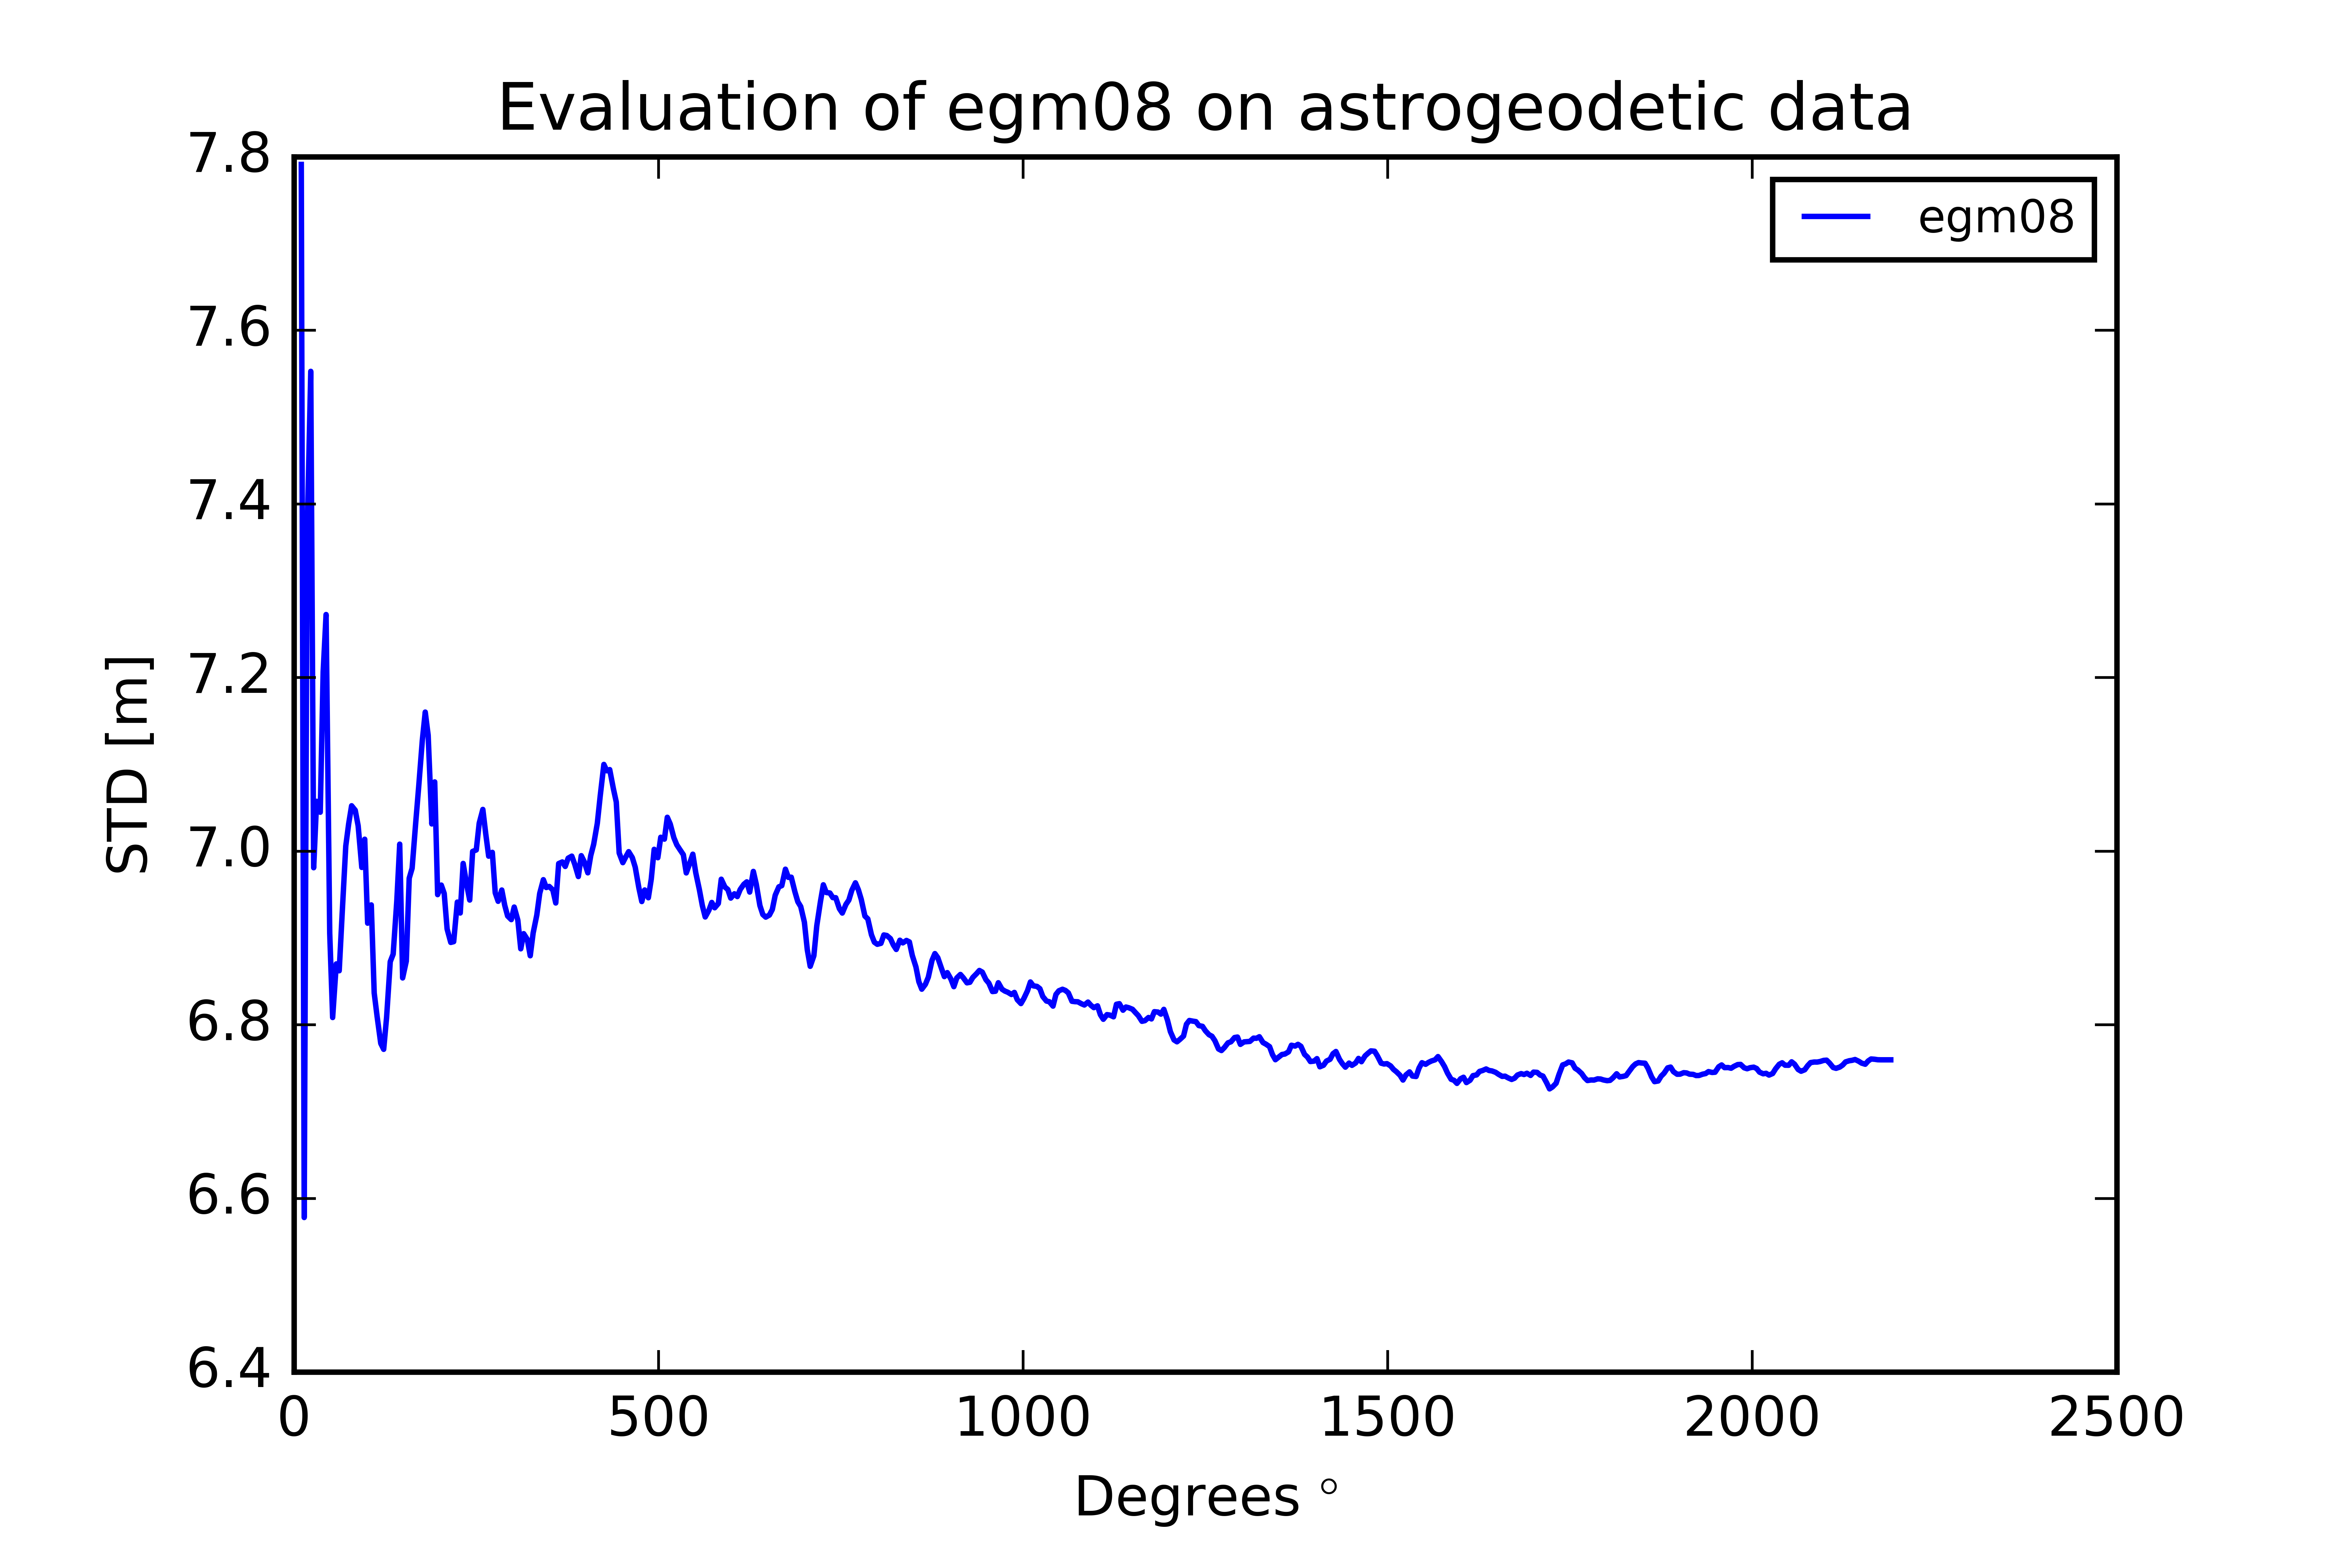
\includegraphics{Figures/egm08_figure.png}
      	\centering
      \end{figure}
      
      
      \begin{figure}[t]
      	\caption{std behaviour with the change of degrees}
      	\label{itu_grace16_figure}
      	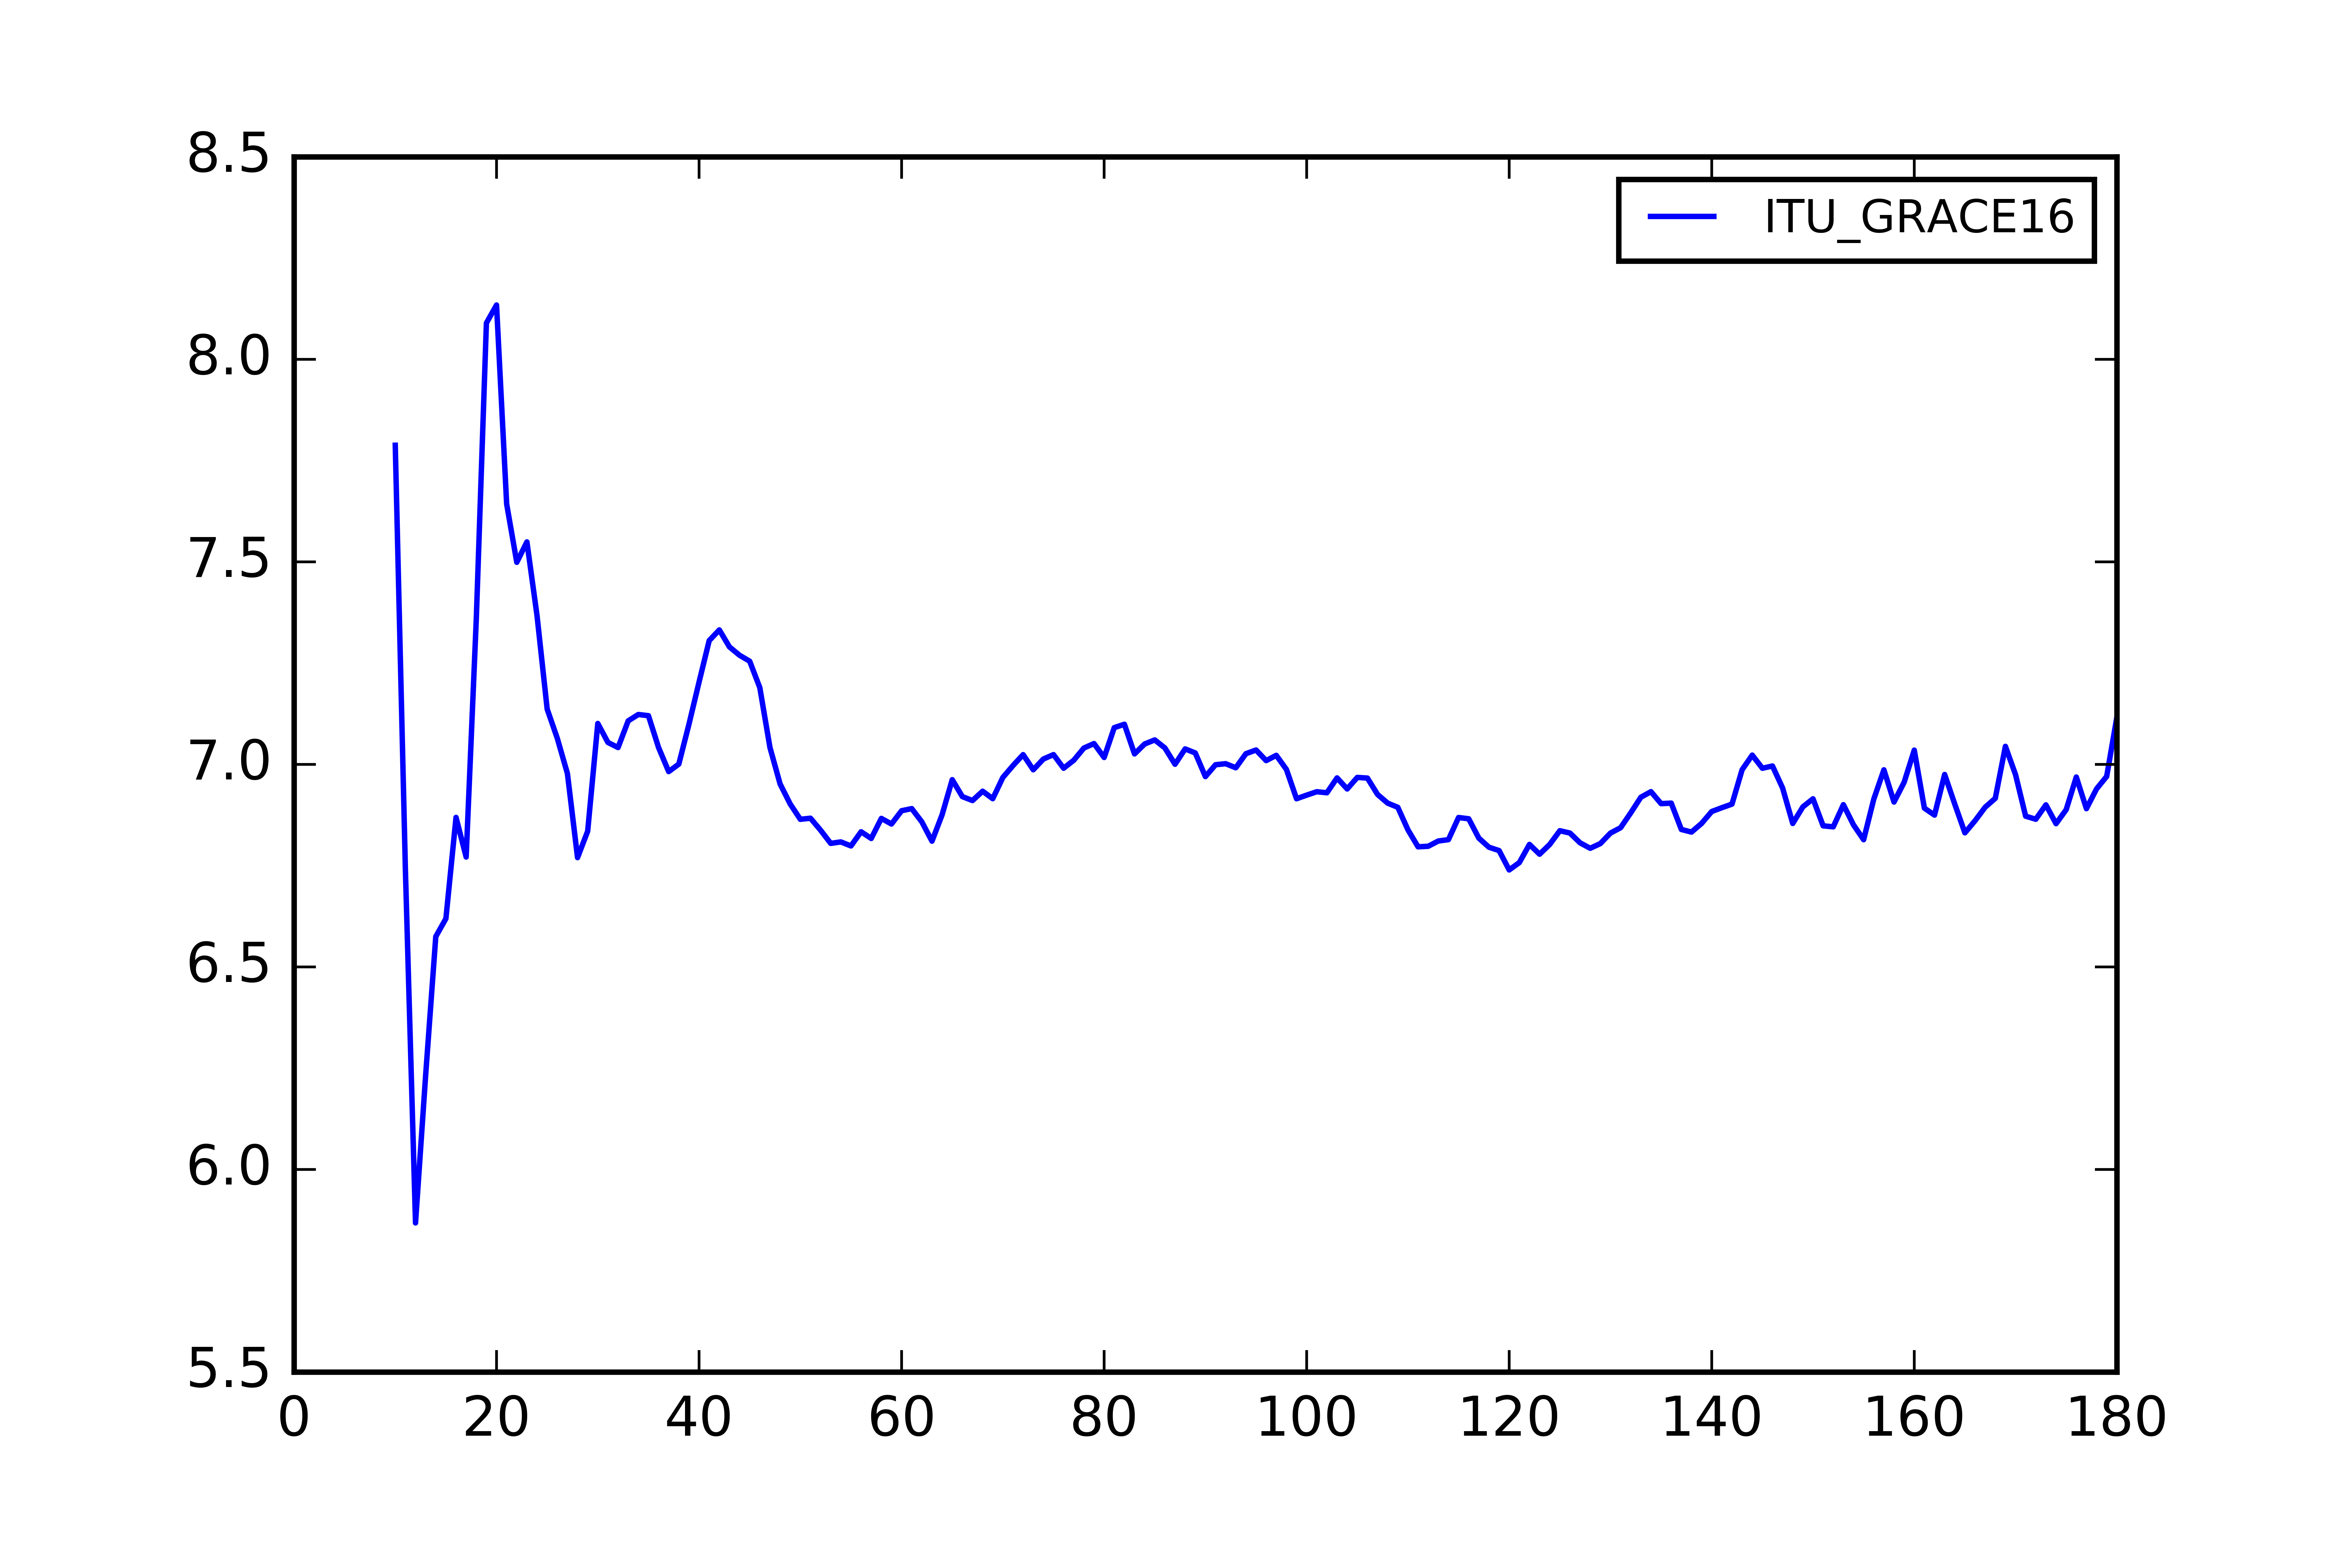
\includegraphics{Figures/ITU_GRACE16_figure.png}
      	\centering
      \end{figure}
      
      
      \begin{figure}[t]
      	\caption{std behaviour with the change of degrees}
      	\label{itu_ggc16_figure}
      	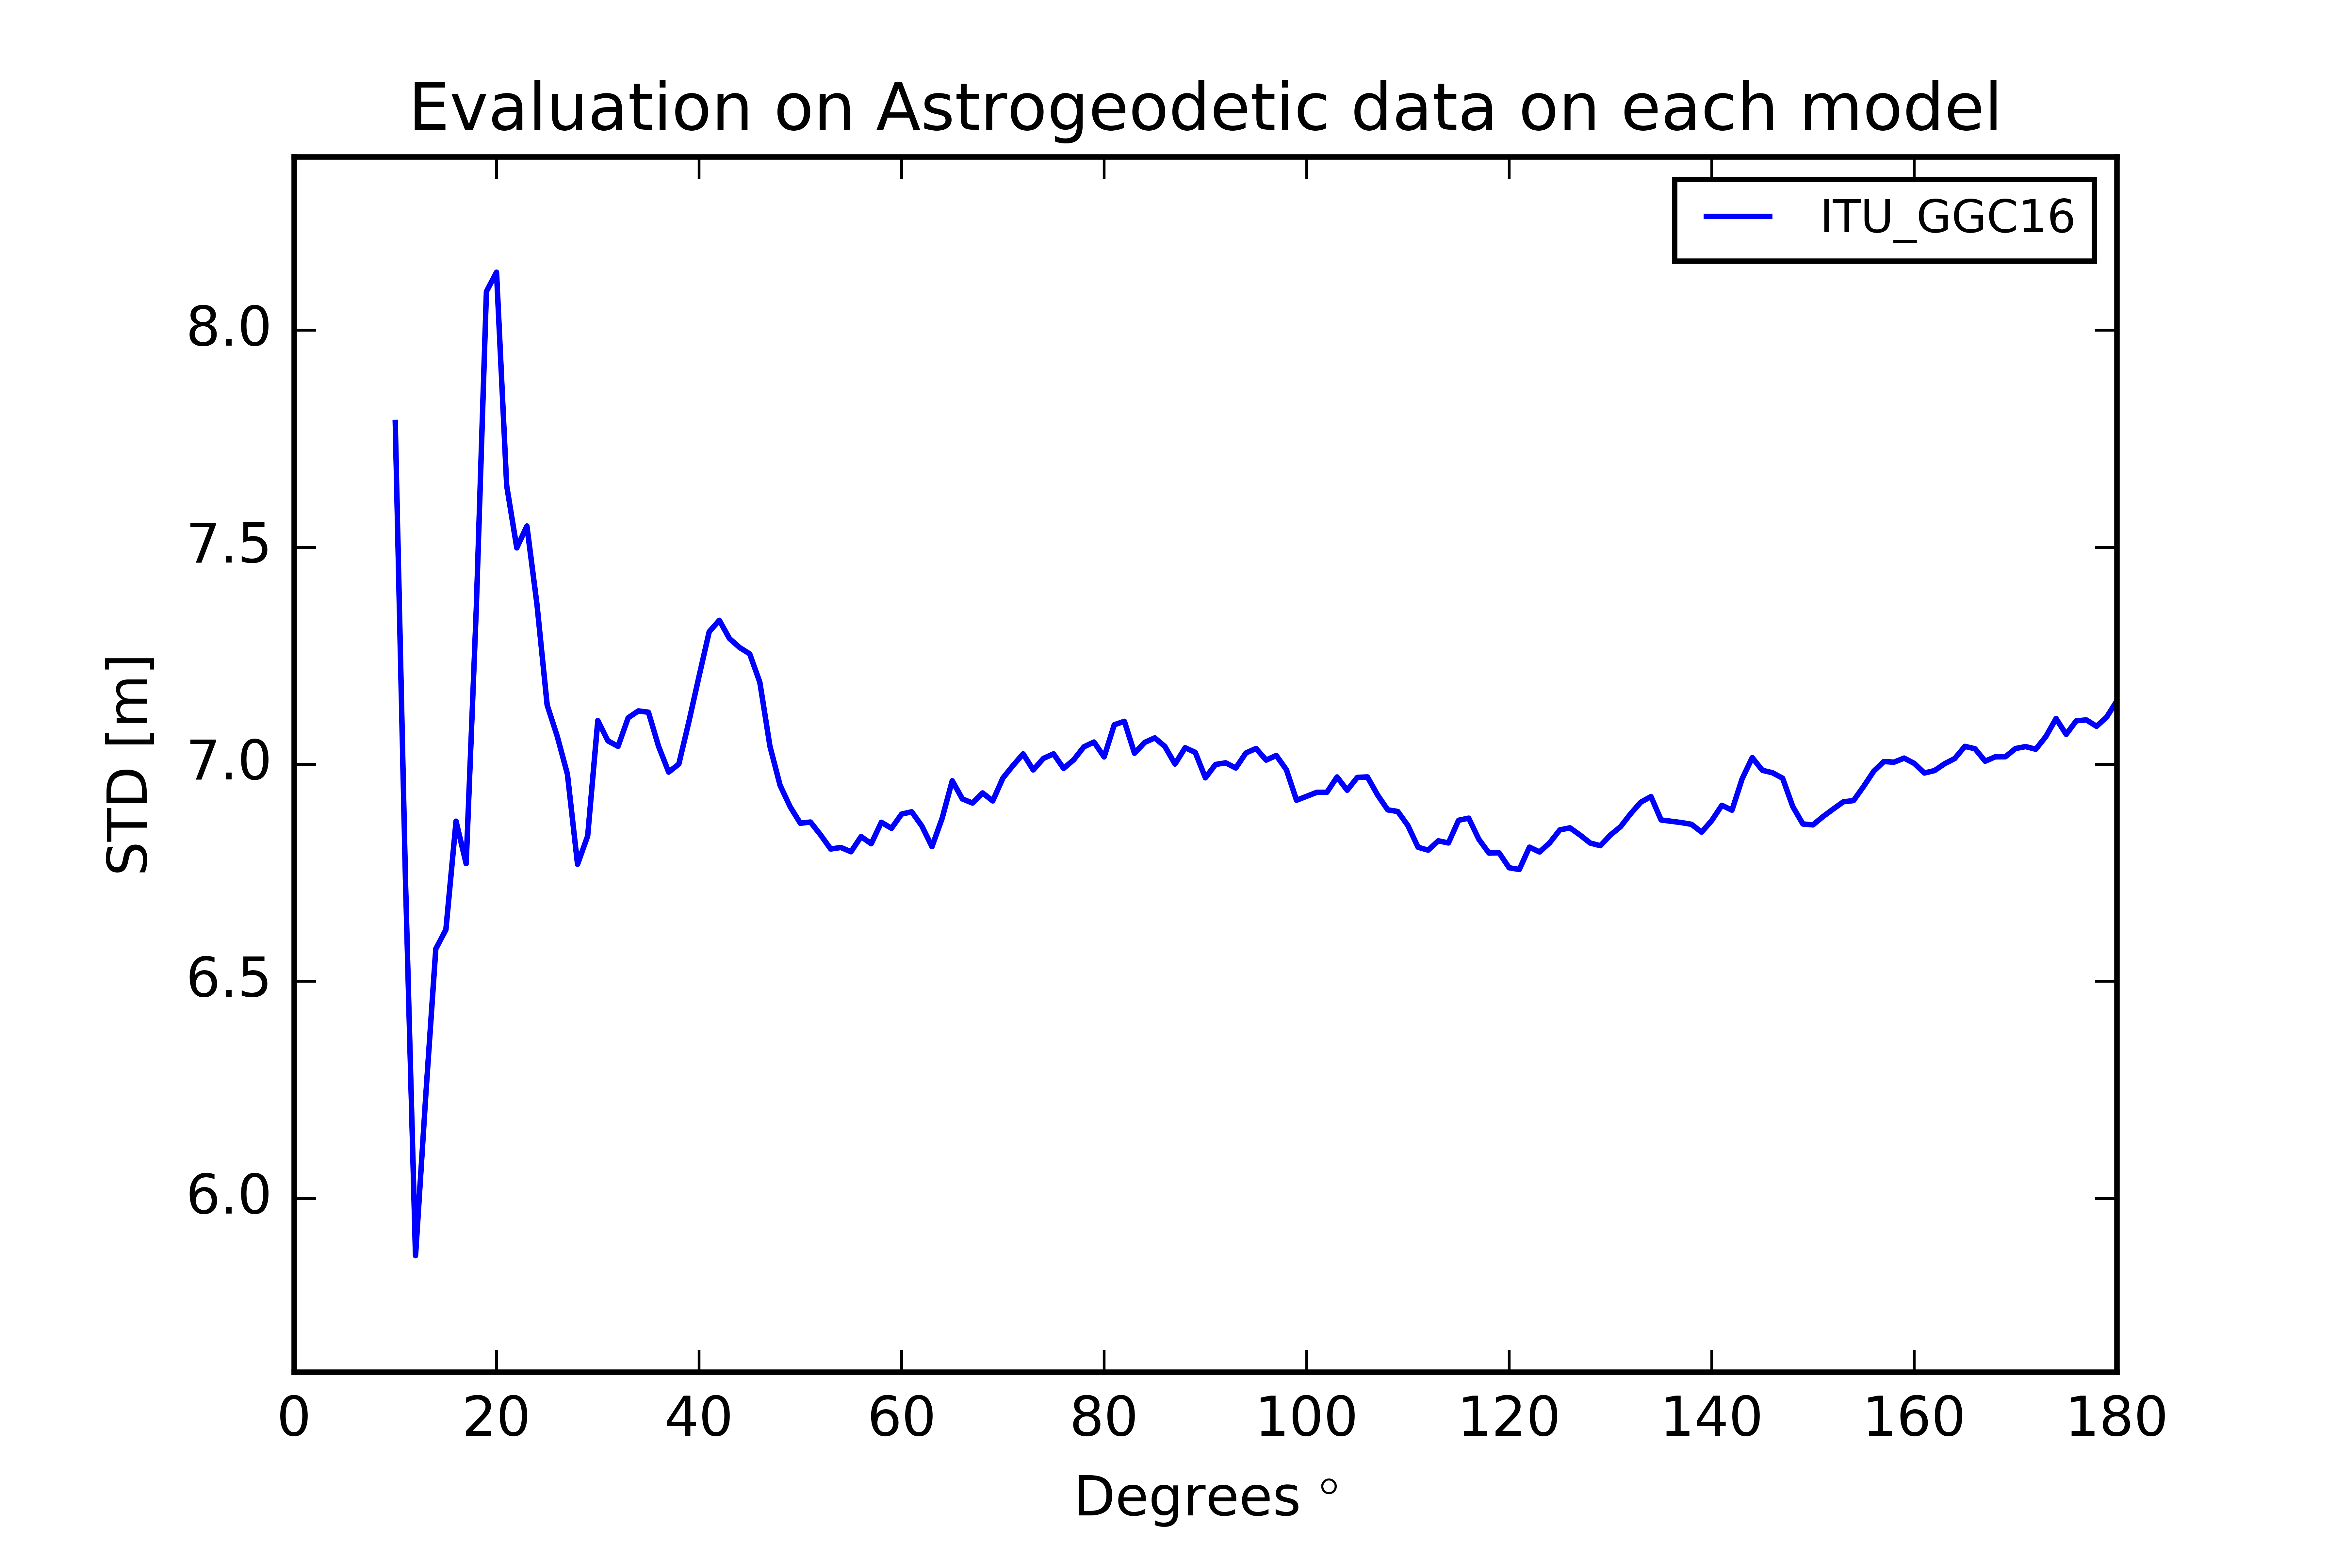
\includegraphics{Figures/ITU_GGC16_figure.png}
      	\centering
      \end{figure}
      
      
      \begin{figure}[t]
      	\caption{std behaviour with the change of degrees}
      	\label{geco_figure}
      	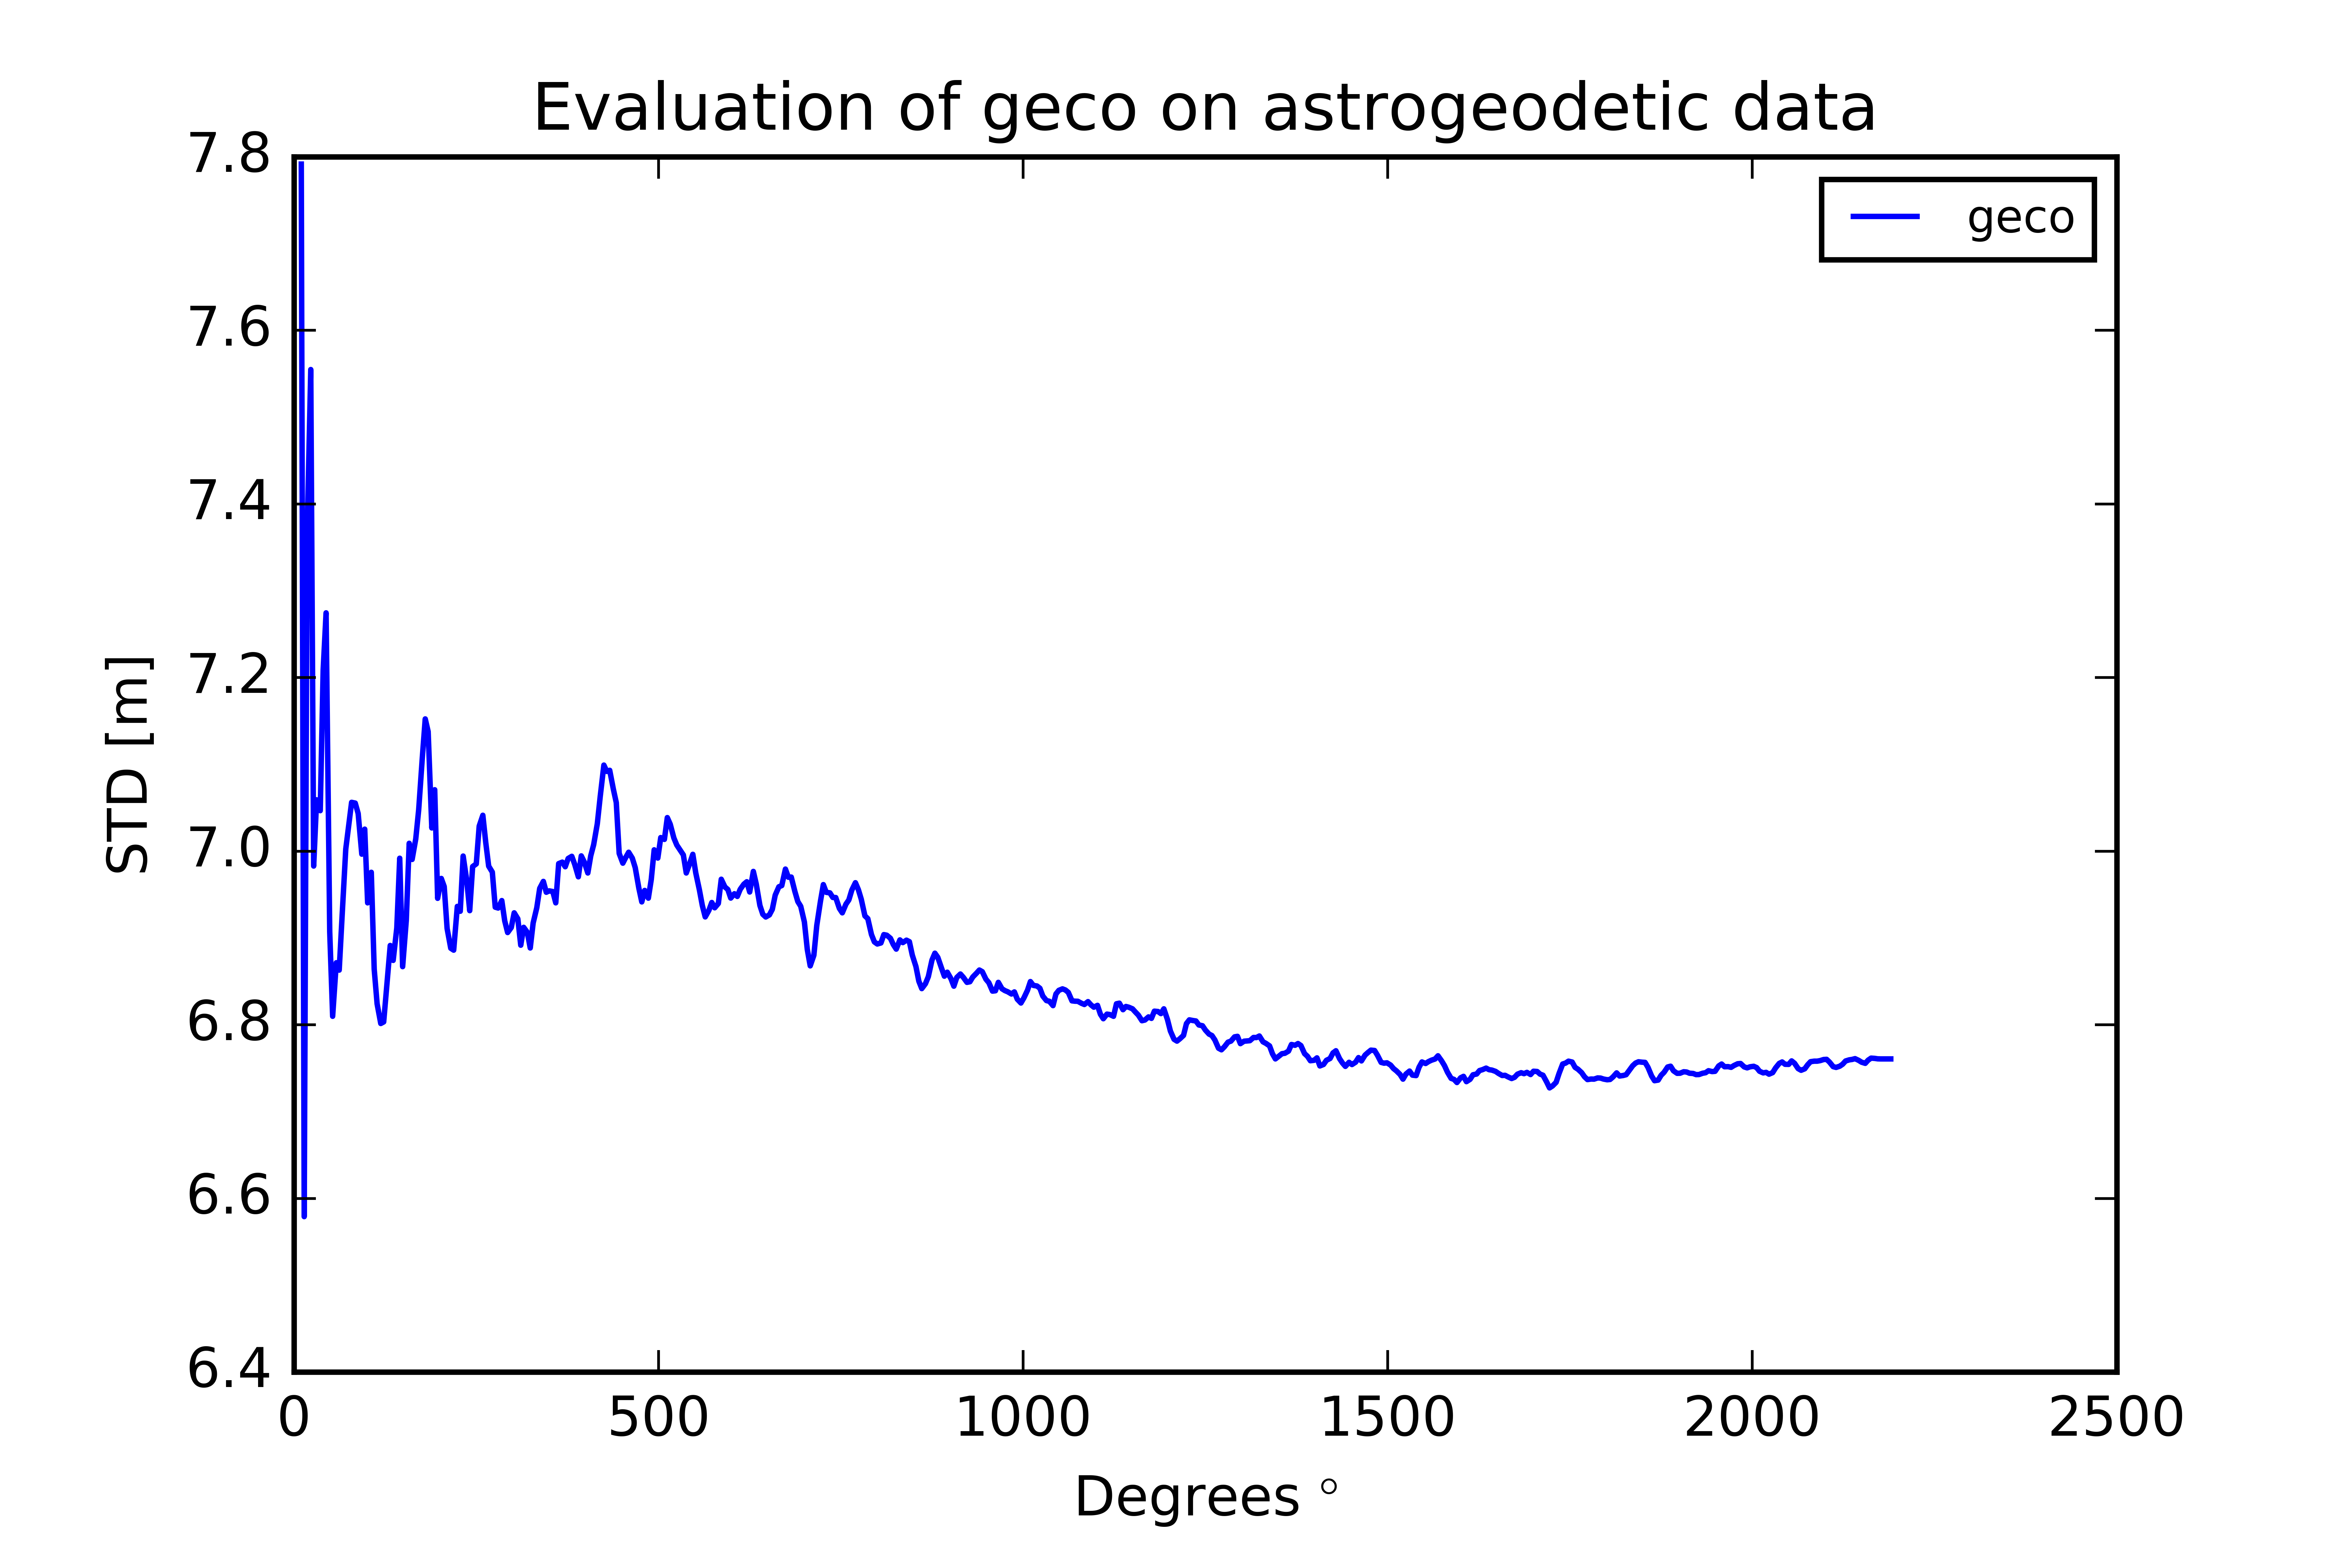
\includegraphics{Figures/geco_figure.png}
      	\centering
      \end{figure}
      
      \begin{figure}[t]
      	\caption{std behaviour with the change of degrees}
      	\label{eigen_6c4_figure}
      	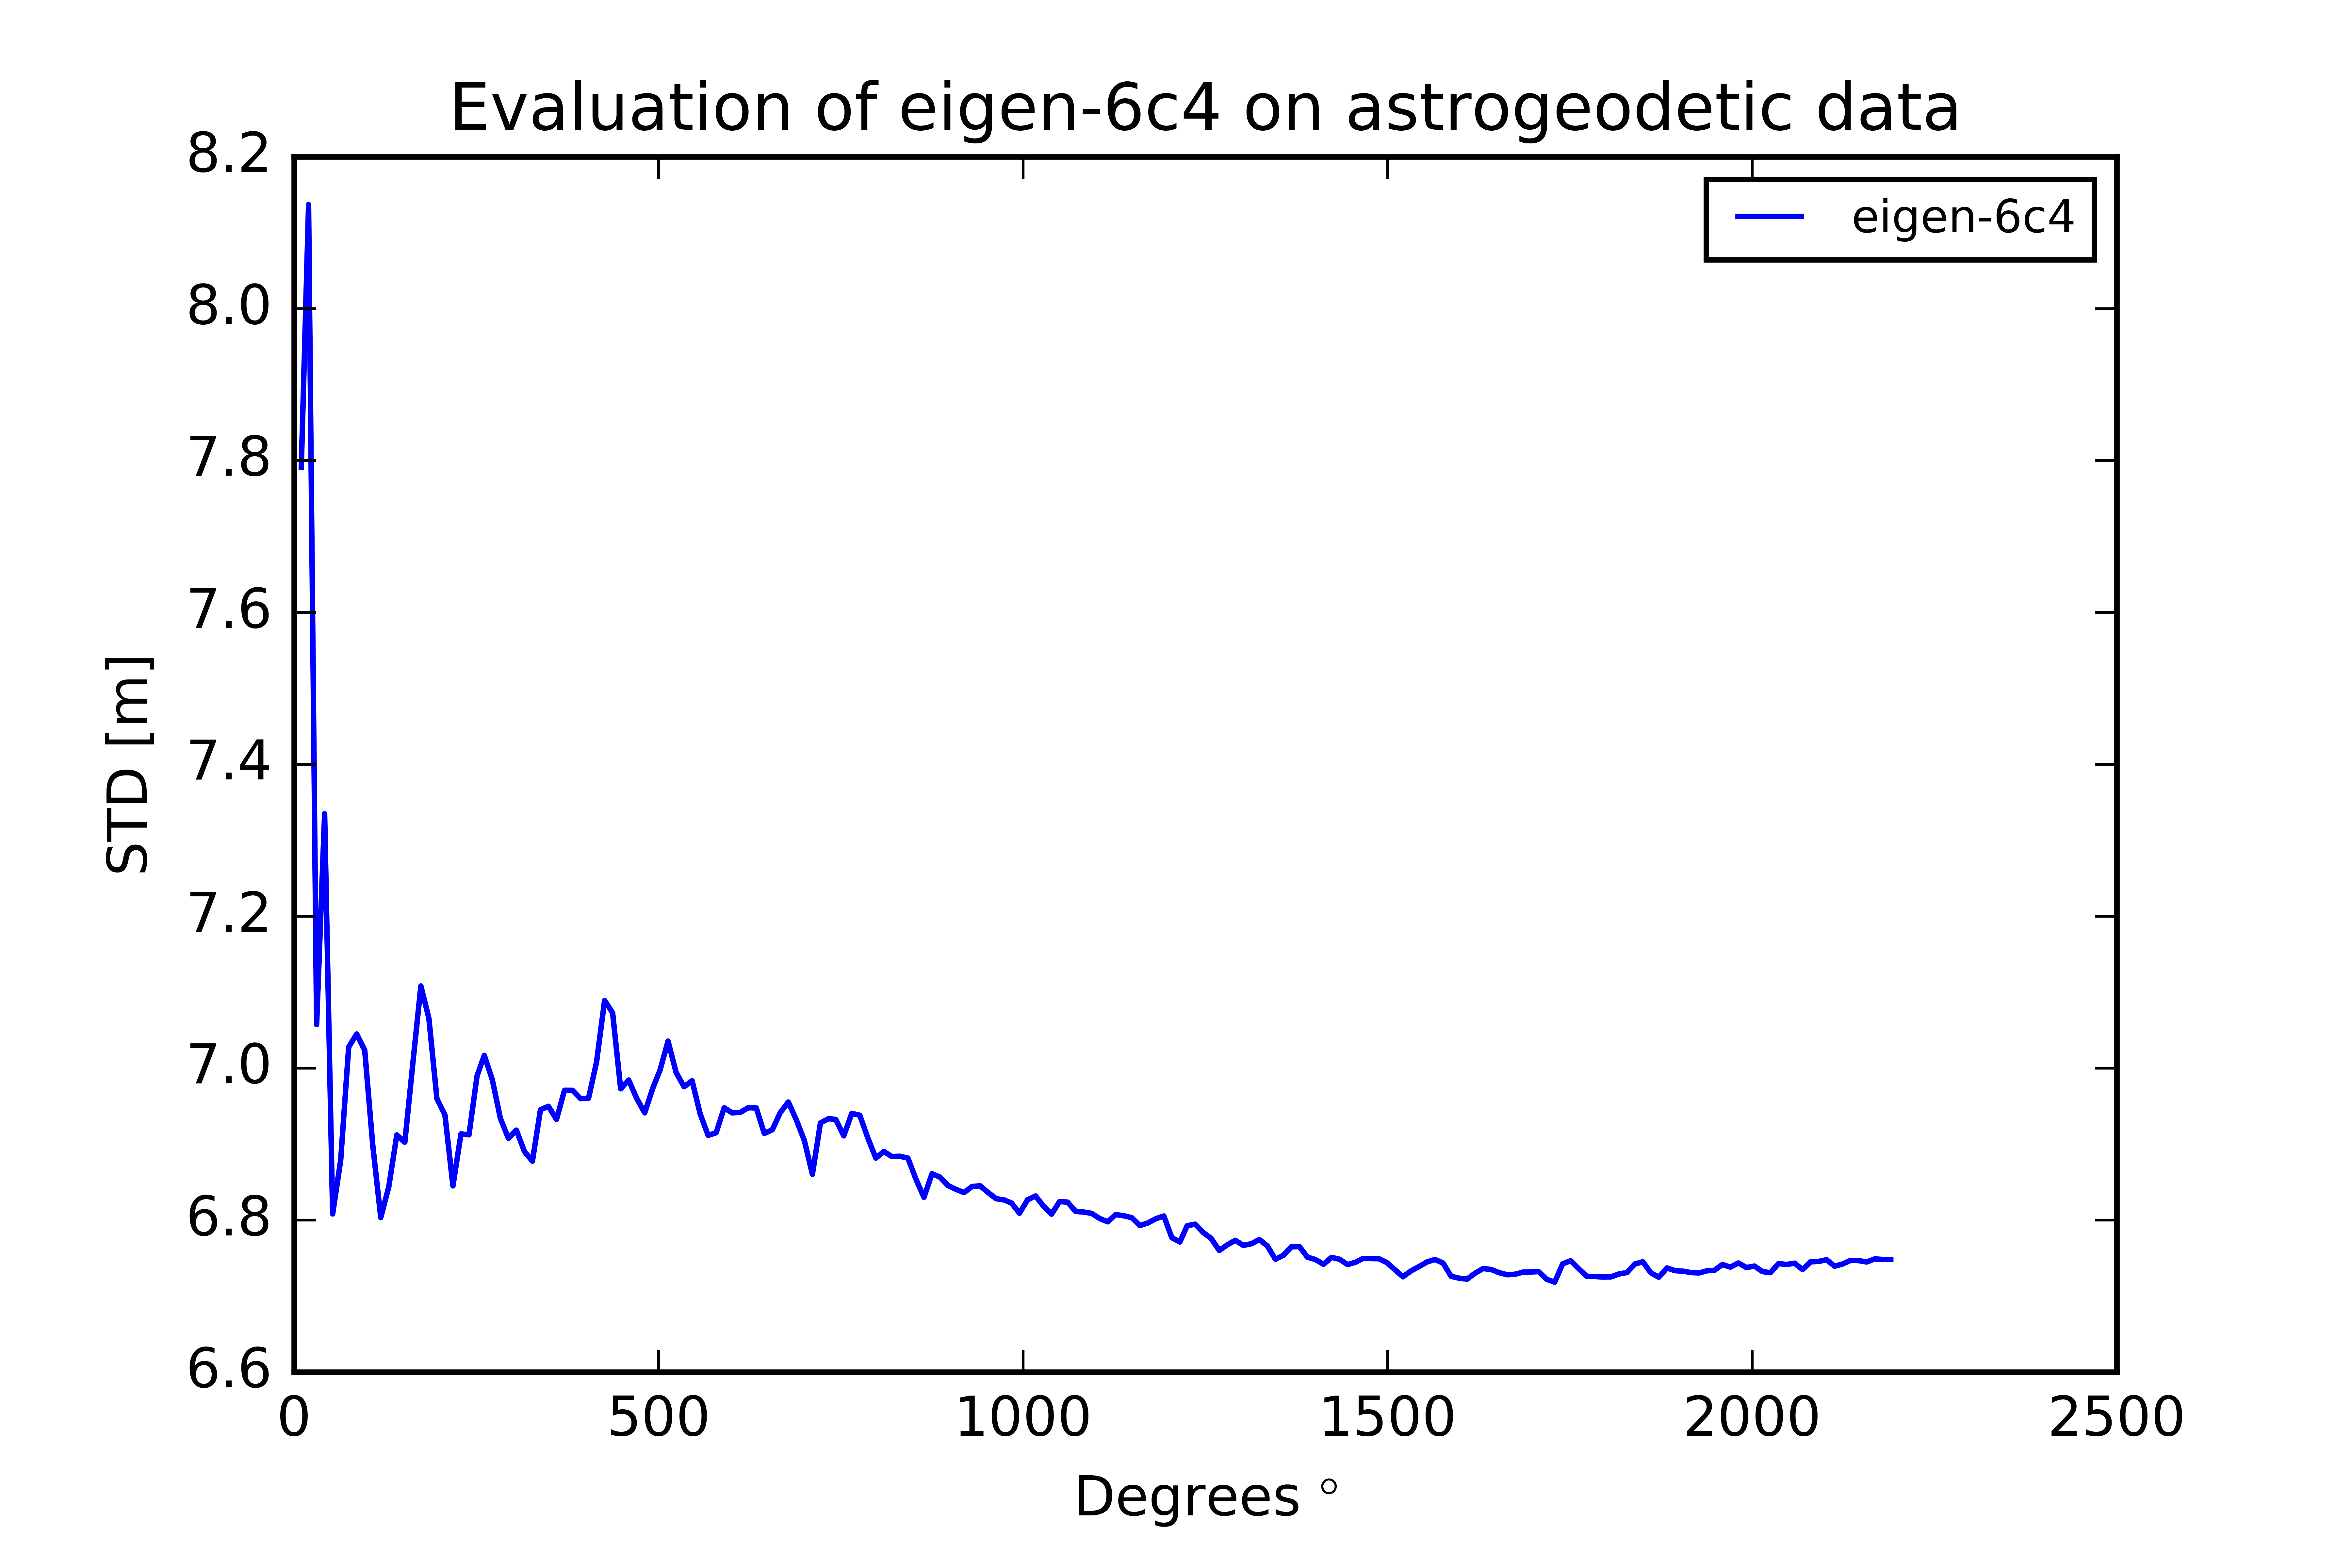
\includegraphics{Figures/eigen-6c4_figure.png}
      	\centering
      \end{figure}